\chapter{Detection and Characterization of Squeezed Light}
\label{ch:5} 
% 24/15 pg
\minitoc

Until now, we have discussed the construction and functioning of the OPO in the classical regime.  We have also seen how pumping the OPO below threshold while sending a vacuum state as input will allow us to produce squeezed vacuum states at the OPO output.  The next step in our task is to measure the quantum states created, and quantify the amount of squeezing produced. 

The detection of quantum states of light is based on the principle that the
current fluctuations produced by light incident on a photodetector are proportional to the quantum fluctuations of the detected light itself.  When we can diminish these fluctuations down to the standard quantum limit, the fluctuations detected by our detector represent what we call \emph{shot noise}.  By ensuring that our detector has the sensitivity to measure light at its shot noise limit, we become capable of also measuring squeezed states when its fluctuations go below this limit.

\section{Balanced Homodyne Detection}
\label{balanced_homodyne_detection} 


\begin{figure}[!htb]
  \centering
  \subfloat[][Direct detection measures intensity level fluctuations of a beam, but provides no access to quadrature information.]{
    \label{fig:fresnel_direct}
    \includegraphics[width=0.38\textwidth]{figures/fresnel_direct} }
  \hspace{30pt} 
  \subfloat[][Homodyne detection projects the quadrature fluctuations of a quantum state onto a local oscillator beam, giving us access to quadrature information.]{
    \label{fig:fresnel_homo}
    \includegraphics[width=0.38\textwidth]{figures/fresnel_homo} } \\
   \caption[Fresnel representation of direct and homodyne detection]{Illustration of direct photodetection vs. homodyne detection. }
   \label{fig:fresnel_detect}
\end{figure}


We have seen that generating squeezed states is a phase-sensitive process, producing states which have quadrature dependant variances.  Using direct photodetection  methods to measure these states however, only provides us with measurements of the intensity fluctuations of the light and offers us no information on the individual field quadratures.  As it is precisely this quadrature noise that characterizes the quantum nature of a squeezed state, we must use another method than direct detection to measure our states.  The method of balanced homodyne detection as we discuss here \cite{bachor2004guide}, allows us to access these different quadratures of the light field, as illustrated in Figure \ref{fig:fresnel_detect}.


To carry out a homodyne detection, we use a 50/50 beamsplitter to mix our signal beam with a mode-matched coherent local oscillator at the same optical frequency, as shown in Figure \ref{fig:homodyne}.  This provides a fixed phase reference for our signal.  On the condition that the local oscillator is much more intense than our signal, such that $\abs{\mathcal{E}_{LO}} \gg \abs{\mathcal{E}_{S}}$, we can treat the local oscillator classically and treat our signal quantum mechanically, linearizing our signal field into the expression $\mathcal{E}_{S} = \avg{\mathcal{E}_S} + \delta \mathcal{E}_s$.  In the case of squeezed vacuum, our signal has low photon number which is approximately zero, and thus we can express our signal as a decomposition of quadrature noises $\delta \mathcal{E}_S = \delta \mathcal{E}^X_S + i\delta \mathcal{E}^Y_S$.

\begin{figure}[ht] 
 \centering
 \includegraphics[width=0.55\textwidth]{figures/homodyne} 
 \caption[Homodyne detection schematic]{An intense phase-scanned local oscillator $\mathcal{E}_{LO}$ mixes with a weaker signal $\mathcal{E}_S$ using a 50/50 beamsplitter, and is sent onto two balanced photodiodes.  By subtracting their photocurrents, we obtain our quadrature signal.}
 \label{fig:homodyne} 
\end{figure}


Upon passing our signal and local oscillator through a 50/50 beamsplitter the output fields satisfy the following relations




\begin{eqnarray}
  \label{eq:homodyne_bs_outputs}
  \mathcal{E}_1 & = & \frac{1}{\sqrt{2}} \left(\mathcal{E}_{LO} e^{i \phi_{LO}} + \delta \mathcal{E}^X_S + i \delta \mathcal{E}^Y_S  \right) \\
  \mathcal{E}_2 & = & \frac{1}{\sqrt{2}} \left(\mathcal{E}_{LO} e^{i \phi_{LO}} - \delta \mathcal{E}^X_S - i \delta \mathcal{E}^Y_S  \right) .
\end{eqnarray}

\noindent
We can then separate our output signals into their real and imaginary parts to obtain
 
\begin{eqnarray}
  \label{eq:homodyne_bs_outputs_reim}
  \mathcal{E}_1 & = & \frac{1}{\sqrt{2}} \left[ (\mathcal{E}_{LO} \cos \phi_{LO}  + \delta \mathcal{E}^X_S ) + i (\mathcal{E}_{LO} \sin \phi_{LO} + \delta \mathcal{E}^Y_S ) \right] \\
  \mathcal{E}_2 & = & \frac{1}{\sqrt{2}} \left[ (\mathcal{E}_{LO} \cos \phi_{LO}  - \delta \mathcal{E}^X_S ) + i (\mathcal{E}_{LO} \sin \phi_{LO} - \delta \mathcal{E}^Y_S ) \right]  .
\end{eqnarray}

\noindent
Now we can detect the light intensity incident on each photodiode using the expression $I_i \propto \mathcal{E}_{i} \mathcal{E}^*_{i} = \abs{\mathcal{E}_{i}}^2$.  Each photodiode will produce a photocurrent $i_i$ proportional to this intensity.  By subtracting these photocurrents, we obtain a resulting photocurrent that is proportional to 

\begin{equation}
  \label{eq:homodyne_photocurrent}
  i = i_{1-2} =  2 \mathcal{E}_{LO} \left[ \delta \mathcal{E}^X_{S} \cos \phi_{LO}   + \delta \mathcal{E}^Y_{S} \sin \phi_{LO}  \right],
\end{equation}

\noindent
with the variance of this difference given by 

\begin{equation}
  \label{eq:homodyne_photo_variance}
  \Delta i^2 \approx 4 \mathcal{E}_{LO}\left(\avg{\delta \mathcal{E}^{2(X)}_{S}} \cos^2 \phi_{LO}  + \avg{\delta \mathcal{E}^{2(Y)}_{S} } \sin^2 \phi_{LO}   \right).
\end{equation}

This shows us that the homodyne detection provides us with a current that is sensitive to the relative phase between our local oscillator and our signal, and is proportional to a linear combination of our quadrature fluctuations.  Furthermore, these equations show that the local oscillator noise term does not contribute in our measurement.  We can express this combination of quadrature fluctuations as our generalized quadrature, $X_\theta$.  Thus we can consider the homodyne detector output as a direct measurement of our signal quadrature, and the photocurrent noise for a given phase can accurately represent our quadrature noise.

In practice there are several critical factors necessary however, in order to assure that the homodyne measurement illustrated here functions properly.


\subsection{Measuring the Rejection Ratio of Subtraction} 
\label{measuring_the_rejection_ratio_of_subtraction} 

In order to verify that the classical noise of the local oscillator is properly subtracted and only the quantum noise is left behind in the photocurrent, we need to measure the rejection ratio of the subtraction circuit.  We carried out this measurement by using an electro-optic modulator to create a 3 MHz intensity modulation of the seed beam passing through the OPO.  We did this by passing the beam through a phase modulator which created a polarization modulation on it, and then we passed it through a PBS cube which created intensity modulations on both output ports of the cube.  These intensity modulations on the two output ports have a relative phase shift of $\pi$ due to energy conservation, thus when beams from both ports are sent into the homodyne detector photodiodes, the subtraction of their photocurrents should give us zero signal.  When one port is blocked, we then obtain a positive signal .  By comparing the ratio  of the one-port signal to the two-port signal, we were able to measure that the photodiode subtraction rejection ratio was at -27dB. 
   




\subsection{Electronic Noise Floor} 
\label{electronic_noise_floor} 

In order to assure that our measurements were not disrupted by external noise sources, we needed to first measure the noise characteristics of our homodyne detector.  The electronic noise floor of the detector provides the lower noise limit, and we needed to assure that it was far enough below the optical shot noise to provide a valid measurement of the squeezing.  We sent 8 mW of light into each photodiode, which was the maximum allowed before saturating the photodiodes.  By observing the photocurrent on a spectrum analyzer, we obtained the measurements shown in Figure \ref{fig:hd_cal}, and observed the shot noise level to be at about -77 dBm.  We then blocked the light entering the photodiodes to measure the dark noise produced by the photodiodes themselves, and found that it was 9 dBm lower than the shot noise level at -86 dBm.  Finally we measured the electronic noise floor of the spectrum analyzer by disconnecting the photodiodes, and found that it had an electronic noise of -89 dBm, which was 3 dBm lower that the dark noise from the photodiodes.  The 9 dBm difference between the shot noise and dark noise from the photodetectors indicates that our local oscillator was intense enough to provide a proper measurement.

\begin{figure}[!htb] 
 \centering 
 \includegraphics[width=0.55\textwidth]{figures/hd_cal} 
 \caption[Homodyne detection noise floors]{Calibration of the homodyne detector noise floors  a) Shot noise from a 16 mW local oscillator at -77 dBm b) Dark noise level of the photodiodes with photodetectors blocked at -86 dBm c) Spectrum analyzer noise at -89 dBm with photodetectors disconnected.} 
 \label{fig:hd_cal} 
\end{figure}


\subsection{Detector Balancing} 
\label{detector_balancing} 

In addition to being electronically balanced, the detectors needed to be optically balanced as well.  We verified the optical balance by observing the AC output on the spectrum analyzer over a 0-5MHz bandwidth.  As a balanced detector should properly subtract classical noise, we used the low-frequency noise level as a measure of the optical imbalance on the high-frequency outputs.  By using a half-wave plate placed in front of the homodyne detector to rotate the polarization, we could control the distribution of power on the two photodiodes, and thus observe the changes to the noise spectrum on the spectrum analyzer, as shown in Figure \ref{fig:homo_balance}.  This allowed us to adjust the optical power distribution in order to minimize the noise traces over the largest bandwidth, thus assuring an optical balance between the two photodiodes.

\begin{figure}[!ht] 
 \centering 
 \includegraphics[width=0.55\textwidth]{figures/balance} 
 \caption[Homodyne detector optical balancing]{We use the noise traces to balance the subtracted AC output for the homodyne detectors while optically balancing the light incident on the detectors.  a) Subtracted output with all light incident on one photodiode b) improved electronic subtraction with 70/30 optical balance c) 50/50 optical balance on photodiodes and optimal electronic subtraction.} 
 \label{fig:homo_balance} 
\end{figure}
 
\subsection{Visibility} 
\label{visibility} 

Performing a homodyne detection requires the signal have a high spatial-mode overlap with a local oscillator.  A poor overlap between the signal and LO modes can be represented as losses in our detection of squeezed states, and thus diminish the amount of squeezing detected.

We performed the visibility measurements by injecting a seed beam into the OPO so that the output light would have the same spatial profile as the squeezed vacuum mode.  We then matched the LO beam power to the OPO signal power, and scanned the relative phase between the two beams by using a piezo attached to the LO path.  This produced interference fringes between the signal and local-oscillator beam, whose amplitude we then measured to quantify the visibility.  The following relation gives us a value of the signal visibility using this fringe measurement \cite{bachor2004guide}

\begin{equation}
  \label{eq:visibility}
  VIS = \frac{I_{max}-I_{min}}{I_{max} + I_{min}} .
\end{equation}

\noindent
For our OPO, we achieved a maximum visibility of up to 99\% between our local oscillator and signal beams, however, typical results were around 95\%.  Our inability to attain more perfect mode overlap is likely due to astigmatism introduced into the signal beam by the OPO cavity angles, which limited the maximum amount of mode overlap we could obtain.


\section{Continuous-Wave Squeezing Measurements}
\label{continuous_wave_squeezing_measurements} 

For the actual measurements, once we had the homodyne detector properly
balanced, we sent 16 mW of power into the local-oscillator so that it would be
much more intense than the OPO signal. We then locked the doubler and OPO at
resonance, set the pump power to 80 mW, slightly below the 90 mW threshold,
and scanned the relative phase between the local-oscillator and the OPO
output.  We then sent the subtracted photocurrent from the homodyne detector
to an Agilient E4411B spectrum analyzer set to zero span mode, at an
observation frequency of 1.5 MHz.  We set the resolution bandwidth to 100 kHz,
the video bandwidth to 100 Hz, and the sweep time to 80 ms.  With these
settings, we were able to observe the amplification and deamplification of the
quadrature noise shown in Figure \ref{fig:sqz_arches} with the deamplification
falling below the shot-noise limit, thus signifying the production of squeezed
states.  We observed $3.0 \pm 0.5$ dB of noise reduction in the squeezed quadratures, and 9 dB of amplification in the anti-squeezed quadrature.  

\begin{figure}[!ht] 
 \centering 
 \includegraphics[width=0.5\textwidth]{figures/arches} 
 \caption[Squeezed vacuum at 1.5 MHz with scanned LO phase]{-3.0 $\pm$ 0.5 dB of squeezed vacuum detected at 1.5 MHz while scanning the LO phase.  The resolution bandwidth is set to 100 kHz and the video bandwidth to 100 Hz.} 
 \label{fig:sqz_arches} 
\end{figure} 

We then analyzed the noise spectrum over a broader bandwidth between 1 MHz and 5 MHz, and observed that the amplitude of the squeezing and anti-squeezing quadratures diminished as we moved up in frequency towards the cavity bandwidth, as shown in Figure \ref{fig:broadband_sqz} 

\begin{figure}[!ht]
  \centering
  \subfloat[Normalized noise variance of the a) squeezed and b) anti-squeezed quadratures from 1 MHz to 5MHz.]{\label{fig:broadband_sqz}\includegraphics[width=0.5\textwidth]{figures/broadband_db} }
  \subfloat[Squeezing measured from 0-500 kHz.  We see that squeezing is preserved all the way down to 30 kHz, making the light compatible for EIT storage in our quantum memory.]{\label{fig:lowfre} \includegraphics[width=0.5\textwidth]{figures/low_freq_db}}
  
  \caption[Broadband and low-frequency squeezing]{Squeezing measurements over a) a broad spectrum, and b) at low frequencies.}
  \label{fig:sqz_broad_low}
\end{figure}
 
We also analyzed the low frequency behavior from 0-500 kHz as shown in Figure
\ref{fig:sqz_broad_low}, in order to determine the lower limit of our squeezing
production.  Producing squeezing at low frequencies is important because we want
to use EIT for storing our state onto the atoms.  The EIT transparency window is
centered around the carrier frequency of our squeezed signal, and has a limited
bandwidth.  Thus, having low-frequency squeezing ensures that we manage to store
the quantum correlations in the limited bandwidth window available through EIT.
We continued to observed -3 dB of squeezing all the way down to 50 kHz, with the
squeezing completely disappearing at 30 kHz.  Given that the electronic
circuitry of our photodiodes imposed a 25 kHz cutoff frequency, we could not observe squeezing more precisely beyond that limit.

\subsection{Comparison With Theory} 
\label{comparison_with_theory} 

We can calculate the theoretical amount of squeezing that should be produced at the OPO output for our OPO configuration, using the relation derived earlier 

\begin{equation}
  \label{eq:opo_variance}
  S_-(\Omega ) = 1 - \frac{T}{T+L}\frac{4 \sigma}{(1+\sigma)^2 + \Omega^2} .
\end{equation}

\noindent
Here, the pump parameter $\sigma$ represents the amount of pump we send as a percentage of the OPO threshold, T is the OPO output coupler transmission, L the intracavity losses, and $\Omega $ the analysis frequency normalized to the cavity bandwidth, which for us was 10 MHz.  For our measurements, we took $\sigma = 0.9$, $\Omega = 0.1$, T = 0.07, and L = 0.02.  This prediction showed us that around -5.8 dB of squeezing should be produced at the OPO output.
 
\subsection{Accounting for Losses} 
\label{accounting_for_losses} 

This prediction of -5.8 dB squeezing production only represents the idealized case given our 2\% of cavity losses, however it does not take into account the inefficiencies of the detection process.

In reality, we have several sources of detection inefficiencies whose presence reduces the amount of squeezing we detect.  These inefficiencies primarily come from optical losses of the beam as it travels from the OPO to the homodyne detector $\eta_{opt}$, the mode mismatch between the squeezed-vacuum and the local oscillator $\eta_{vis}$, and the imperfect quantum efficiency of our photodiodes $ \eta_{quant}$.  We can thus assign a global efficiency to our entire detection process with 

\begin{equation}
  \label{eq:overall_efficiency}
  \eta_{det} \; = \; \eta^2_{vis} \cdot \eta_{quant} \cdot \eta_{opt}.
\end{equation}                   

\noindent
For our experiments, we can set a visibility estimate of 96\%, an estimate 5\% for our optical path losses, and an estimate of 90\% for the quantum efficiency of our photodiodes.  This results in an overall detection efficiency of $\eta_{det} = 0.9\cdot 0.96^2 \cdot 0.95 \approx 0.8$.  With this value in place, we can now derive an estimate of the amount of squeezing that we will realistically measure by using our beamsplitter model for losses given by \req{eq:sqz_noise_increase}

\begin{equation}
  \label{eq:loss_variance}
  S^{det}_{-}(\Omega) = S^{opo}_{-}(\Omega) \; \eta_{det} + (1 - \eta_{det}).
\end{equation}

\noindent
This expression gives us the detected noise measurement of our signal as a function of the detection efficiency, and the noise at the OPO output.  By using the values estimated above, we predict a detection closer to -3.9 dB of squeezing, as plotted in Figure \ref{fig:sqz_meas_pred}. 

\begin{figure}[!ht] 
 \centering 
 \includegraphics[width=0.55\textwidth]{figures/sqz_meas_pred} 
 \caption[Estimation of squeezing production in our OPO]{Squeezing prediction with a 7\% output coupler, $P_{Pump}$ at 90\% of threshold, and 2\% cavity losses with a) real detection inefficiencies of $\eta_{det}=0.8$  and b) perfect detection efficiency $\eta_{det}=1$.} 
 \label{fig:sqz_meas_pred} 
\end{figure}

This estimation corresponds well to the measured results once we take into account optical losses and detection inefficiencies.  It thus shows that we have an accurate estimation for the operating parameters of our system.

\section{Quantum State Tomography}
\label{quantum_state_reconstruction} 

As discussed in Chapter \ref{ch:2}, the density matrix $\dens$ provides us with the most complete representation of a quantum state, allowing us to calculate any quantity for our system that is predictable by quantum mechanics.  We also saw earlier how the Wigner function provides a representation of the information contained within the density matrix.  Quantum State Tomography (QST) is a technique that allows us to take the projective quadrature measurements of our system, and reconstruct the full density matrix and Wigner function for our quantum state.  In this section, we will see how we carried out this task, leading to a complete characterization of our squeezed light.

\subsection{Homodyne Measurements} 
\label{homodyne_measurements} 

The first step in QST is to build up a large amount of projective quadrature measurements.  As we have seen earlier, the balanced homodyne detector provides us with a direct measurement of the quadrature fluctuations of the light

\begin{equation}
  \label{eq:bhd_quad}
    I_2 - I_1 = \hat{\mathcal{E}}_\phi = \frac{1}{\sqrt{2}} (\ani e^{-i \phi } + \crea e^{i \phi })  ,
\end{equation}

\noindent
where $\phi $ represents the relative phase difference between the squeezed signal and the local oscillator.  For a given local oscillator phase, the measured quadrature follows a probability distribution which is a projection of the states Wigner function onto the linear combination of the state's two quadratures, which we can represent using the generalized quadrature $x_\theta$.  Thus the homodyne measurement provides us with direct probability distributions of quadratures of the state, and by scanning the local oscillator phase, we can measure these probability distributions for all phase angles in $[0, 2\pi]$.


\subsection{Tomographic Reconstruction} 
\label{tomographic_reconstruction} 

Once we have measures for the quadratures for all of the phases, we can begin to use reconstruction techniques to estimate the density matrix for our state.

Historically, the technique of the Inverse Radon Transform \cite{leonhardt1997measuring} was used to reconstruct the state from the measured quadrature distributions.  However, this approach was shown to be prone to creating artificial artifacts in the reconstructed state, could lead to unphysical results, as well as being very sensitive to errors leading to instabilities in the data.  We thus decided to use an approach which improves on some of the flaws of the inverse Radon transform.

 
  
\subsection{Maximum Likelihood Estimation} 
\label{maximum_likelihood_estimation} 

The approach we decided to use, Iterative Maximum Likelihood Estimation (MLE), was outlined by \cite{PhysRevA.61.010304} and \cite{PhysRevA.63.040303}, and developed into an algorithm by \cite{lvovsky2004}.
 
MLE works by beginning with an arbitrary starting point, and iteratively converging towards an estimation of the density matrix that would have the highest probability of producing our observed dataset \cite{RevModPhys.81.299}. The estimation process assures that we have a physically meaningful state at the end, without the artificial artifacts introduced by the inverse Radon transform.

We can begin to quantify this approach by starting with the definition of \emph{likelihood}, where the likelihood of our state is given by the product of all the marginal probabilities

\begin{equation}
  \label{eq:quantum_likelihood}
  \mathcal{L}(\dens) = \prod p(\ket{x_{\theta}, \theta}).
\end{equation}

\noindent
The individual probabilities here represent the probabilities of obtaining a given quadrature measurement $x_{\theta}$ at a given phase angle $\theta $.  This expression tells us that we need to record enough data to build up accurate probability histograms of each generalized quadrature, at multiple phase angles so that we can cover the entire phase space.  The algorithm then introduces an operator $\hat{R}(\dens)$

\begin{equation}
  \label{eq:r_operator}
  \hat{R}(\dens) = \sum^N_{i=1} \frac{\Pi(x_{\theta_i}, \theta_i)}{p(x_{\theta_i}, \theta_i)} ,
\end{equation}

\noindent
where $\Pi(x_{\theta_i}, \theta_i)$ are the projectors constructed from a set of basis states $\ket{x_{\theta_i}, \theta_i}$.  We can then use the following update relation to estimate the density matrix that is incrementally more likely to have produced the dataset.

\begin{equation}
  \label{eq:maxlik_update}
  \rho' = \frac{\hat{R}(\dens)\dens \hat{R}(\dens)}{Tr \left( \hat{R}(\dens) \dens \hat{R}(\dens) \right)} .
\end{equation}

\noindent
By iterating over Equation \ref{eq:r_operator} and Equation \ref{eq:maxlik_update} many times, we can eventually converge towards a reasonable estimation for our state $\dens$.


\subsection{Experimental Implementation} 
\label{experimental_implementation} 

  The first step in performing the tomography involved acquiring a digital representation of the photocurrent from the homodyne detector, which contained all of the information necessary to reconstruct our state.

We sent the homodyne difference photocurrent to a ZFL-500LN-BNC Low Noise amplifier, which amplified our signal by 5 dB, allowing us to slightly increase our signal-to-noise ratio.  We then sent the photocurrent to a computer-hosted NI PCI-5122 digitizer containing 256 MB of RAM, which we used to perform a running acquisition of the photocurrent at 100 MHz, with 14-bit resolution.  We triggered the beginning of the card acquisition on the rising edge of the TTL controlling the local oscillator sweep, and arranged the sweep frequency so that we could obtain a $2\pi$ phase rotation during the acquisition window.  Using this card, we recorded 1 million data points of shot noise by blocking the OPO output, and 1 million data points of squeezed quadrature noise while sweeping the local oscillator phase.  This allowed us to obtain the digital representations of the photocurrents shown in Figure \ref{fig:dig_noise}.

\begin{figure}[!ht]
  \centering
  \subfloat[Shot noise showing uniform photocurrent variance.]{\label{fig:shot_noise}\includegraphics[width=0.5\textwidth]{figures/shot_noise} }
  \subfloat[Squeezed vacuum showing quadrature fluctuation amplification and deamplification as we scan the LO phase.]{\label{fig:sqz_noise}\includegraphics[width=0.5\textwidth]{figures/sqz_noise} }
  
  \caption[Digitized photocurrents of shot noise and vacuum squeezing]{Digitized photocurrents of a) shot noise and b) squeezed vacuum recorded at 100 MS/s using a NI PCI-5122 digitizer.}
  \label{fig:dig_noise}
\end{figure}

With these photocurrent acquisitions, we then normalized the squeezing points to the shot noise, and manually associated phase reference points to the squeezed data in order to create $x_\theta$, $\theta $ pairs for all of the data points.  We then divided the $0-2\pi$ phase points into 100 bins, sorted the quadratures by phases, and calculated the average quadrature value for each phase bin.  Next, we needed to reconstruct our projectors $\Pi_{nm}(x_i, \theta_i )$ from the quadrature data, and thus needed to select a set of basis states to represent them.  We selected the Fock basis, with the infinite Fock space truncated to 10 photons.  We then used the quadrature data to construct the projectors using the expression \cite{lvovsky2004}

\begin{equation}
  \label{eq:fock_projectors}
  \Pi_{nm}(x_i, \theta_i ) = e ^{i(n-m)\theta_i}\left(\frac{1}{\pi}\right)^{1/2} \frac{1}{\sqrt{2^{n+m}n!m!}}e^{-x^2_{i}} H_n(x_{i})H_m(x_{i}),
\end{equation}

\noindent
where the $H_n(x_i)$ are the $n^{th}$ order Hermite polynomials, and the $x_i$ and $\theta_i$ are the quadrature and phase data.  With these projectors, we then ran the MLE algorithm for 100 iterations, and obtained a reconstruction of the state's density matrix.
 
\begin{figure}[!ht] 
 \centering 
 \includegraphics[width=0.5\textwidth]{figures/density_sqz} 
 \caption[Density matrix estimated using iterative MLE] {Density matrix of up to 10 photons estimated using iterative MLE method.} 
 \label{fig:density_sqz} 
\end{figure}
 
We see from Figure \ref{fig:density_sqz} that 10 photons are enough to perform our reconstruction, as there appears to be an almost zero probability of higher numbers of photons appearing.  The noise calculations for this state indicate a measure of 1.97 dB $\pm$ 0.05 dB of squeezing for this acquisition, which shows consistency with our spectrum analyzer measurements.

We also generated the Wigner functions for our state as shown in Figure \ref{fig:wigner_shot_sqz}, which show visually that we have managed to produce and reconstruct a state with asymmetric noise variances in its two quadratures, with one quadrature having a sub shot noise variance.

\begin{figure}[!ht] 
 \centering 
 \includegraphics[width=0.75\textwidth]{figures/wigner_shot_sqz} 
 \caption[Wigner functions for shot noise and squeezed state]{MLE reconstructed Wigner functions for a) shot noise and b) squeezed state.  This corresponds to around 2.4 dB of squeezing.} 
 \label{fig:wigner_shot_sqz} 
\end{figure}



\section{Creation of Pulses of Squeezed Light}
\label{creation_of_pulses_of_squeezed_light} 

Once the tools for the generation and characterization of squeezed light were put into place, we needed to properly interface the light with the atomic system for storage.  The atomic storage medium itself imposed a set of constraints on the means of storing the light.  Firstly, we wanted to carry out many repetitions of the storage in a finite sized atomic medium, thus we needed to create pulses of squeezed light from the continuous OPO-generated source.  The limited EIT storage lifetime also required that we create short pulses, thus we sought to create pulses sized between 1 $\mu s$ - 5 $\mu s$  in length.  In creating such short pulses, we also needed to verify that the frequency components which were contained in the pulse would still preserve the squeezing.  Because we would be sending pulses of squeezed vacuum, we would not be able to directly detect the pulse arrival.  Yet, knowledge gained from prior experiments \cite{CviklinskiPhD} had shown us that the EIT would require a precise timing of pulses to within 100 ns precision, thus the system that created the pulses would have to be stable, and have extremely low jitter, allowing us to predict the pulse arrival time to within 100 ns.  Additionally, we wanted to run the experiment as quickly as possible, thus we sought to have a high repetition rate for the pulse creation.  We predicted that the MOT would need around 18 ms to properly prepare the atomic cloud in between each storage run, thus we wanted to present a squeezed pulse to our MOT every 25 ms, which set another constraint on our pulse generation rate.

Another aspect that we needed to carefully consider was the fact that the squeezing in our pulse would be destroyed by any losses or inefficiencies in the pulse generation or detection process.  Thus, we need a system to create the pulses which would minimize the losses, and we needed to properly time our detection as to maximize the measurement of squeezing, and minimize the measurement of the vacuum contributions.

Given our restrictions concerning the timing precision and optical losses, we considered two different techniques to generate the squeezed light pulses.  AOMs are typically used to generate light pulses and offer a timing precision of around 100 ns, but often create optical losses of 20\% on each passage of the beam through the AOM.  Optical choppers add no losses to a beam as they either completely block, or completely allow the passage of a beam of light, however as they are mechanical devices, they offer much less timing precision.  In the following sections, we will discuss our efforts to create optical pulses using these two approaches.


\subsection{AOM Implementation} 
\label{aom_implementation} 

We initially wanted to avoid using an AOM to create the pulses, as we expected from measurements on similar AOMs that in the optimistic case, we would add 20\% losses to our beam per AOM.  After searching for high-performance models, we found an upgraded model of the AOMs that we previously used (MT110-A1-IR) from AA Optoelectronics.  This upgraded model had a specification for 99\% transmission at our wavelength, and 92\% beam diffraction into the 1st order mode, as well as a rise time of less than 200 ns for our pulse edges, thus we could minimize our losses during the pulse measurements.  Our measurements confirmed we could obtain characteristics with our system that approached these specifications, with 96\% transmission and 93\% diffraction per AOM.  Thus, we decided to use two of them in a 0-order configuration as illustrated in Figure \ref{fig:aom_pulse_block}, where activating them would diffract the light away from our pathway leaving only $7\% \cdot 7\%  \approx 0.5\%-1\%$ of the original squeezed light in the optical path.  We considered that this would be effective, as the 99\% losses would effectively destroy the squeezing in the small amount of light that passed when we diffracted the beam, and we would only experience 8\%-10\% losses when the beam was transmitted.

\begin{figure}[!ht] 
 \centering 
 \includegraphics[width=0.55\textwidth]{figures/aom_pulse_block} 
 \caption[Schematic for AOM optical pulse generation]{We send a TTL signal each AOM's RF driver to alternate between the on and off states, deviating thee optical path to create an optical pulse.} 
 \label{fig:aom_pulse_block} 
\end{figure}


The AOM offered the timing precision and repeatability of pulse creation and triggering that we had come to expect with previous AOM usage from other experiments.  The optical pulses were created only when we sent a TTL signal to the AOMs, and thus created a simple mechanism for creating the experimental timing sequence.





\subsection{Optical Chopper Implementation} 
\label{optical_chopper_implementation} 

As we wanted to attempt to minimize losses as much as possible, we also explored usage of an optical chopper.  One issue that we needed to consider when using an optical chopper were the pulse edges created by the mechanical operation of the chopper.


\subsubsection{Optical Detection Losses Due To Pulse Edges} 
\label{optical_losses_due_to_pulse_edges} 
One problem that arises in the measurement of squeezed light pulses is that by creating the pulses using a chopper, we create sections of the pulse where the normalized light intensity is less than 1 during the pulse rise and fall times.  We can consider these segments as periods when vacuum noise mixes with our squeezing, thereby increasing the amount of noise in our measurement.  Thus, we can simulate these periods as undergoing optical losses.  As we want to minimize the losses experienced during the detection of our squeezing, we would ideally keep the pulse rise and fall times to a minimum.

We can begin modelling these losses with a simplified model of our pulse passing through our optical chopper.  Suppose that we have a slit of width $l$ rotating at speed $\omega$ at a distance of $r$ from our disc center.  We can approximate that $r \gg l$, and we have a uniform intensity over our beam cross section instead of gaussian.  This allows us to express the pulse as composed of the segments shown in Figure \ref{fig:chopper_pulse_fig} 

\begin{figure}[!ht] 
 \centering 
 \includegraphics[width=0.65\textwidth]{figures/chopper_pulse_fig} 
 \caption[Illustration of a pulse generated by an optical chopper]{Model of a pulse generated by chopper with long rise and fall times.  The normalized intensity $I_0$ falls below 1 for the periods $t_{rise}$ and $t_{fall}$.} 
 \label{fig:chopper_pulse_fig} 
\end{figure}

\noindent
where

\begin{eqnarray}
  \label{eq:pulse_time_segments}
  t_{rise} = t_{fall} = \frac{\omega_0}{\pi r f}  & \text{and} & t = \frac{l + 2\omega_0}{2 \pi r f}  ,
\end{eqnarray}

\noindent
where $f$ is the chopper rotation frequency and $\omega_0$ is the beam radius.  If we consider our optical losses experienced through the rise/fall times as time averaged losses over the entire detection period, we can derive a simple model of the losses by considering them as the difference between the time averaged intensity of an ideal pulse, and that of a real pulse

\begin{equation}
  \label{eq:pulse_losses}
  \text{losses} = I_0\frac{t - \int^t_0 \rho(t') \, dt'}{t} , 
\end{equation}

\noindent
where the real pulse intensity envelope is given by a time dependent function $\rho(t)$.  Now by normalizing our intensity to 1, and using our assumption of uniform cross section intensity, we can see that the losses evaluate to

\begin{eqnarray}
  \label{eq:bs_pulse_losses}
  \text{losses} = 1 - \frac{t-t_{rise}}{t} = 1 - \frac{l}{l+2 \omega_0}  & \text{or} & \eta^2_{trans} = \frac{l}{l+2 \omega_0}  ,
\end{eqnarray}

\noindent
which shows that the losses only depend on our spot size relative to the aperture width.  We can then use our loss expression in the beamsplitter model for losses to evaluate the loss effect on a given level squeezing using \req{eq:sqz_noise_increase}





\subsubsection{Real Pulse Envelope}
\label{real_pulse_envelope} 

With respect to using an optical chopper, preliminary calculations showed us that if we wanted to produce a pulse of 1 $\mu s$ light, we could accomplish that by passing the light through a 50 $\mu m$ slit, attached to a disc rotating at around 200 rotations per second.

We can develop a more realistic model for our pulse envelope $\rho(t)$ by dropping our assumption of a uniform beam intensity over the cross section.  We can begin by expressing the intensity as a gaussian profile normalized to 1

\begin{equation}
  \label{eq:spot_gaussian}
  I_0(r) = \sqrt{\frac{2}{\pi \omega_0^2}} e^{-\frac{2r^2}{\omega_0^2} }, 
\end{equation}

\noindent
where $r$ describes our distance from the beam center.  We can then define the intensity of a beam after passing through the chopper, as $I_{chop}$, which is given by integrating our gaussian profile over our chopper slit width

\begin{equation}
  \label{eq:i_chop}
  I_{chop}(x) = \int^{x+l/2}_{x-l/2} I_0(r) \; dr.
\end{equation}

\noindent
We can then plot \req{eq:i_chop} from the points before the beam enters the slit, until after it passes, to obtain a realistic profile of the effect of the chopper.  Simulating this with a spot radius of $\omega_0 = 10 \mu m$, a chopper frequency of 200 Hz, a disc radius of 46 mm, and a slit size of 50 $\mu m$ produces the pulse profile shown in Figure \ref{fig:real_chopper_pulse} with a 1 $\mu s$ width, conforming to our requirements.

\begin{figure}[!ht] 
 \centering 
 \includegraphics[width=0.55\textwidth]{figures/real_chopper_pulse} 
 \caption[Chopper pulse model with gaussian profile]{1 $\mu s$ pulse modeled using gaussian intensity profile.  Created by sending a 10 $\omega_0=10 \mu m$ beam through a 50 $\mu m$ aperture on a r=46 mm disc rotating at 200 Hz.} 
 \label{fig:real_chopper_pulse} 
\end{figure}





\subsubsection{Slit Selection}
\label{slit_selection} 

We thus choose to use a Thorlabs Fixed Vertical Slit, model S50R, similar to that shown in Figure \ref{fig:thorlabs_slit}.  As these slits had a fabrication size of 50 $\mu m$  $\pm$ 3 $\mu m$, they provided a much more reliable aperture size than we could produce on our own.

\begin{figure}[!ht] 
 \centering 
 \includegraphics[width=0.30\textwidth]{figures/slit_200_h} 
 \caption[Thorlabs 200 $\mu m$ slit]{An example 200 $\mu m$ Thorlabs slit, removed from its steel housing} 
 \label{fig:thorlabs_slit} 
\end{figure}

\subsubsection{Beam Focusing}
\label{beam_focusing} 

In order to properly fit the beam through the slit, it needed to be highly focused.  One danger of passing squeezed light through an aperture is that an improperly sized beam can have its squeezing destroyed due to diffraction losses.  Given that we wanted to use a 50 $\mu m$ slit, in order to lose less than 1\% of power from diffraction losses, we calculated the waist size of the beam that could be passed through the slit of width D using \cite{Siegman86}

\begin{equation}
  \label{eq:siegman_diffraction}
  D = \pi \omega_0.
\end{equation}

This indicated that a waist with a 10 $\mu m$ radius would be sufficiently small. We purchased a high quality doublet lens from Newport with a focal length of f = 38.7 mm, which we used to focus the beam down to this size.   We picked the doublet shape as to minimize the amount of aberrations that we would introduce onto the beam as any aberrations would make it difficult to obtain a high mode overlap  upon recombination with the local oscillator.  We mounted these lens onto a Newport M-UMR5.11 translating stage, so the could have micrometric control over the beam waist position.  This proved critical, as the beam's waist had a sensitivity of a few mm.

\subsubsection{Chopper Selection}
\label{chopper_selection} 

With the slit selected, we needed to mount it to a rotating disc in order to create our optical chopper.  We selected the Scitec instruments 310CD optical chopper, shown in Figure \ref{fig:chopper_open}, which could rotate a disc up to 400 rps, thus twice our required speeds.  Its specifications for stability indicated a < 0.02\% variation in the chopper speed, which suggested that jitter would not be a problem for our experiment.  The company provided solid un-machined discs, which we used to create our own custom disc design.  Another important aspect, is that the chopper contained an integrated optical fork which output a TTL signal every time the disc would pass.  This would allow us to signal the creation of an optical pulse, and prepare our experiment.

\begin{figure}[!ht] 
 \centering 
 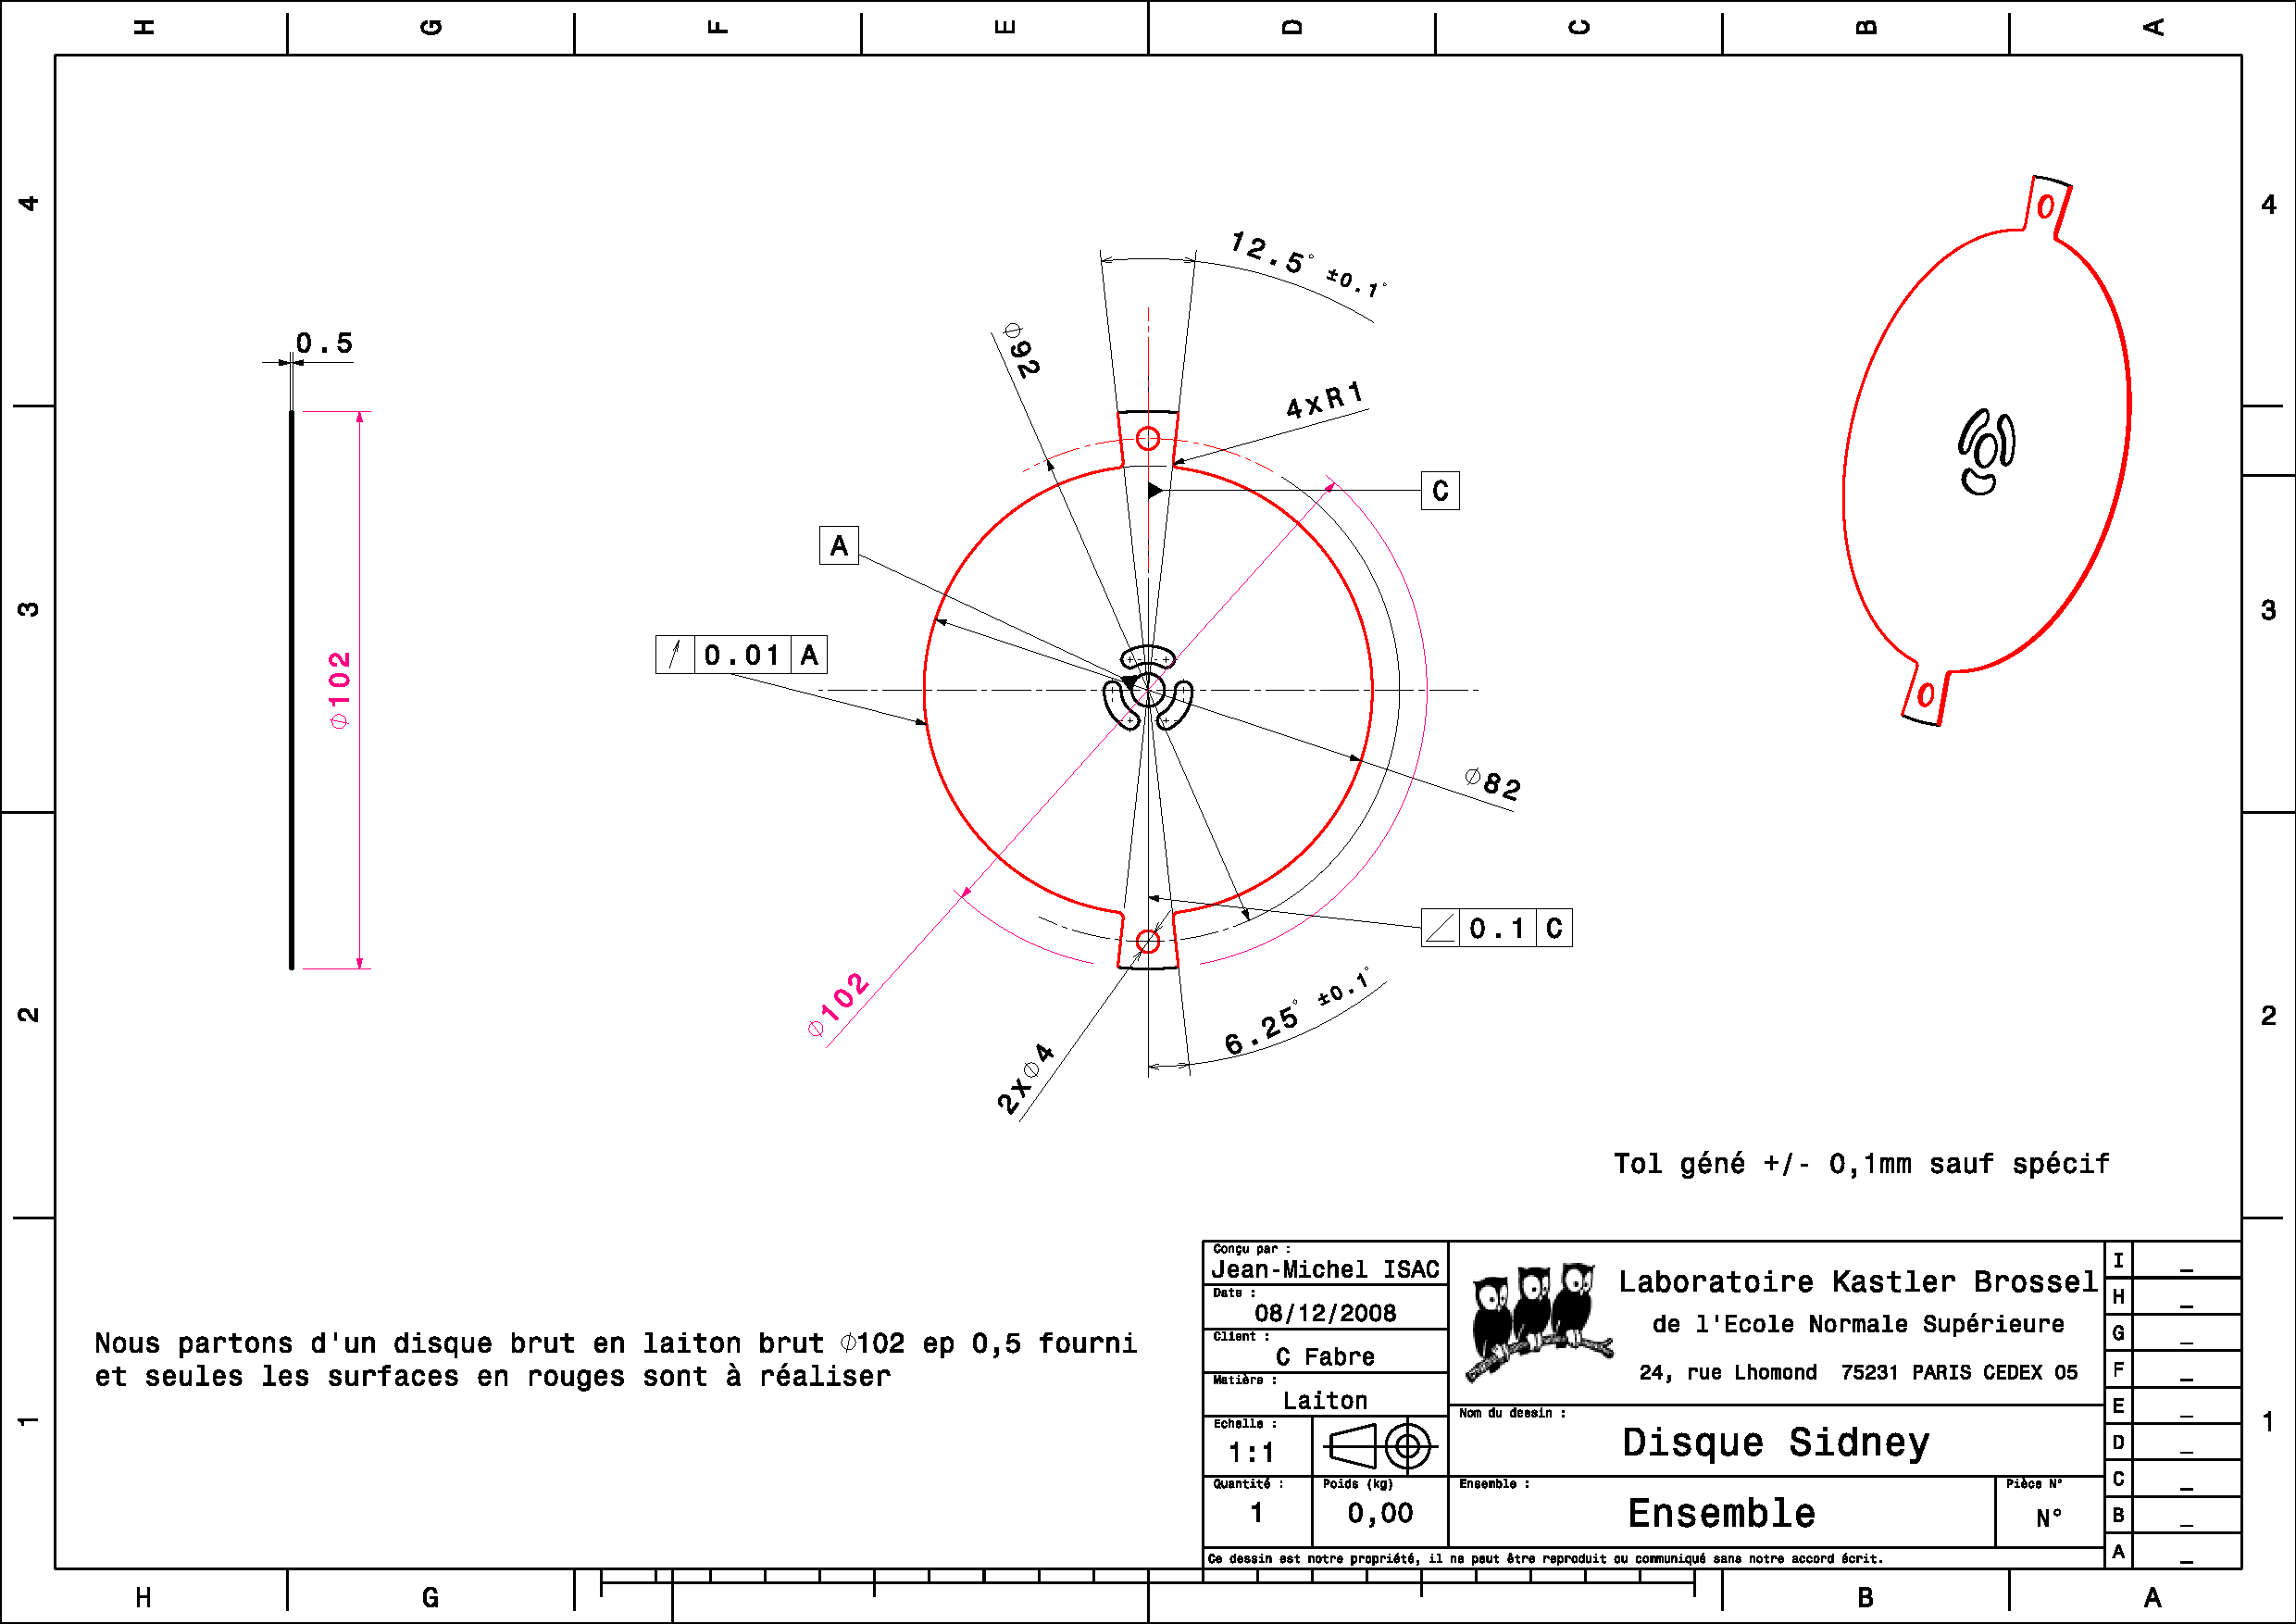
\includegraphics[width=0.45\textwidth]{figures/chopper} 
 \caption[Scitec 310CD Chopper]{Scitec 310CD chopper with protective case opened to show optical fork.} 
 \label{fig:chopper_open} 
\end{figure}


\subsubsection{Rotating Disc}
\label{rotating_disc} 

We then sought to mount the slits onto the discs provided.  For the memory experiment, we wanted the light to follow a particular on/off sequence.  During a long period A, we wanted the squeezed beam to pass into the atoms, which would allow us to track the relative phase between the squeezed beam and the local oscillator.  Then for a shorter period B, we wanted to cut off the squeezing creating a \emph{dark time} in order to finalize the preparation of the MOT.  Finally, we would present the actual pulse in C, after which the sequence would relaunch.  Figure \ref{fig:timing_diagram} illustrates this concept.

\begin{figure}[!ht] 
 \centering 
 \includegraphics[width=0.55\textwidth]{figures/timing_diagram} 
 \caption[Optical timing sequence for pulse generation]{Optical squeezed vacuum pattern needed for storing a pulse in the quantum memory.  We track the phase at A (25 ms), prepare the memory at B (100 $\mu s$), and store the pulse at C (1 $\mu s$).} 
 \label{fig:timing_diagram} 
\end{figure}

Our proposed solution to create this sequence was to construct a slotted disc with protruding teeth.  By placing the Thorlabs slit into the disc, the light could pass by the disc for the majority of the time, be blocked by the protruding tooth, and reappear when aligned with the tiny slit, producing the pulse.  


\subsubsection{Disc Balancing}
\label{disc_balancing} 

As the disc was rotating at 200 rps, the slightest imbalance could introduce instabilities into its rotation, and thus create jitter.  Thus, we constructed a symmetric disc having protrusions on both sides in order to maintain the balance.  

Introducing a second slit to the disc preserves its balance, however because no two slits are exactly identical, the size of the pulse created from the second slit has no relation to the first, which means that we can't use both pulses for the experiment.  The simplest solution that we developed was to just ignore the TTL produced from the second slit, so that it would not trigger the experiment.  In Chapter \ref{ch:7}, we will discuss the FPGA techniques used to create a TTL decimator, which allowed us to selectively ignore certain signals.  As we only used one of the slits, we placed a 200 $\mu m$ slit into the second side in order to have a more versatile disc for experimenting with different pulse sizes.


\subsubsection{Disc Geometry}
\label{disc_geometry} 

We determined that the slit needed to be placed at a 46 mm radius from the disc center, and that the tooth needed to cover an angle of 12.45\textdegree .  This would allow us to produce pulses of around 1 $\mu s$, and dark periods of around 100 $\mu s$ for a 4 ms rotation period at 200 rps.  We had the disc cut from our design shown in Appendix \ref{appendix:chopper_disc_diagram} by a commercial agency, and the end result produced the disc shown in Figure \ref{fig:chopper_disc}.

\begin{figure}[!ht] 
 \centering 
 \includegraphics[width=0.30\textwidth]{figures/chopper_disc} 
 \caption[Custom designed disc for optical chopper]{Customized disc designed to hold both 200 $\mu m$ and 50 $\mu m$ Thorlabs slits.} 
 \label{fig:chopper_disc} 
\end{figure}


\subsubsection{Pulse Measurements}
\label{pulse_measurements} 

We then mounted the chopper assembly and securely fastened it to the table, and locked the OPO with a seed beam injected so that we could directly observe the pulses produced on the squeezed light path.  As the chopper's rotation speed and stability exceeded our initial estimated requirements, we managed to produce well-formed pulses with widths down to 450 ns.  Furthermore, by comparing the pulse amplitude to the amplitude of the light not passing through the slit, such as in Figure \ref{fig:200um}, we can see that our tight focusing allowed us to avoid any diffraction losses. The pulses shown in Figure \ref{fig:chopper_pulses} illustrate our results.
  
\clearpage
\begin{figure}[!ht]
  \centering
  \subfloat[][3 $\mu s$ ]{
    \label{fig:3us}
    \includegraphics[width=0.41\textwidth]{figures/chopperzoom50100} }
  \subfloat[][1.5 $\mu s$ ]{
    \label{fig:1.5us}
    \includegraphics[width=0.41\textwidth]{figures/chopperzoom50200} } \\
  \vspace{-10pt}
  \subfloat[][1.0 $\mu s$ ]{
    \label{fig:1us}
    \includegraphics[width=0.41\textwidth]{figures/chopperzoom50300} }
  \subfloat[][780 ns]{
    \label{fig:780ns}
    \includegraphics[width=0.41\textwidth]{figures/chopperzoom50400} } \\
  \vspace{-10pt}
  \subfloat[][640 ns]{
    \label{fig:640ns}
    \includegraphics[width=0.41\textwidth]{figures/chopper50500} } 
  \subfloat[][520 ns ]{
    \label{fig:520ns}
    \includegraphics[width=0.41\textwidth]{figures/chopperzoom50600} } \\
  \vspace{-10pt}
  \subfloat[][450 ns]{
    \label{fig:450ns}
    \includegraphics[width=0.41\textwidth]{figures/chopper50700} } 
  \subfloat[][1.6 $\mu s$ - shortest pulse created with 200 $\mu m$ slit]{
    \label{fig:200um}
    \includegraphics[width=0.41\textwidth]{figures/chopper200800side} }
  \caption[Optical chopper pulse measurements]{Optical pulses created using the 50 slits $\mu m$ \subref{fig:3us} - \subref{fig:450ns} and 200 $\mu m$ slits \subref{fig:200um} }
  \label{fig:chopper_pulses}
\end{figure}

\clearpage

Thus, the chopper did manage to create the stable short pulses that we required, however there were a few critical drawbacks.
\subsubsection{Noise}

Due to the chopper's high rate of speed, it created a large amount of noise which filled the entire room, disrupting other sections of the experiment.  We tried to minimize this noise by using smaller holes to inject the light into the chopper, and we installed the entire apparatus in the plexiglass box shown in Figure \ref{fig:chopper_box} that was lined with lead and foam.  This completely removed the noise at rotational speeds up to 600 Hz.

\begin{figure}[ht] 
 \centering 
 \includegraphics[width=0.45\textwidth]{figures/chopper_box} 
 \caption[Acoustic isolation box for dampening chopper noise]{Plexiglass box used to attenuate the acoustic noise from the chopper.  The interior of the box was coated with a foam/lead material to absorb the sound.  Silent performance up to 600 Hz.} 
 \label{fig:chopper_box} 
\end{figure}

 
\subsubsection{Vibrations}
\label{vibrations} 

A more critical problem however, arose from the vibrations transmitted from the chopper to the table.  This would be expected since the chopper was securely fastened to the table, however as a result, these vibrations prevented us from maintaining the OPO locked at resonance.  We thus attempted to attenuate the vibrations by placing a sandwich of isolating material underneath the chopper as shown in Figure \ref{fig:chopper_sandwich}.  Through trial and error, we chose a mixture of aluminum, lead, styrofoam and sorbothane, as well as placed sheets of lead beneath the OPO itself for increased attenuation.


\begin{figure}[!hbt] 
 \centering 
 \includegraphics[width=0.45\textwidth]{figures/chopper_sandwich} 
 \caption[Chopper vibration isolation stack]{Isolation sandwich used to attenuate chopper vibrations, consisting of aluminum, lead, styrofoam, and sorbothane.} 
 \label{fig:chopper_sandwich}  
\end{figure}
   
\subsubsection{Jitter}
\label{jitter} 

When using the chopper, the entire experiment needed to be triggered from the chopper pulse because the exact time when the pulse would be created was uncertain.  This posed a problem because as stated earlier, EIT storage required us to have a 100 ns predictability of the pulse arrival time.  Despite our successes in removing the acoustic noise and attenuating the chopper vibrations, problems of pulse jitter re-arose and proved to be a final problem.  When we fixed the chopper rigidly to the table, the jitter was on the order of several ns.  However, when we used the isolation to attenuate the mechanical vibrations, we could no longer securely fasten the chopper to the table, and thus its movement created pulse jitter of 500 ns.  This uncertainty was much too large for us to properly use the EIT protocol, and it made it impossible for us to predict to within 100 ns when the next pulse would arrive - thus ruining the timing for the pulse detection and triggering the experiment.  



%% \subsection{Quantum Tomography of Pulsed Squeezing} 
%% TODO
